%% Supplementary material for "What source validation cannot see".
%% Compiled separately from main.tex; it therefore cannot cross-reference the
%% article's labels, and refers to it by section name instead.
\documentclass[a4paper,fleqn]{cas-dc}
\usepackage[authoryear]{natbib}
\setlength{\emergencystretch}{2em}
\graphicspath{{../figures/}}

\begin{document}
\let\WriteBookmarks\relax

\shorttitle{Supplementary material}
\shortauthors{P. Singh and P. Singh}

\section*{Supplementary material}

Supplement to \emph{What source validation cannot see: an affine adaptation
audit for cross-corpus speech emotion recognition}.

Everything here comes from the same frozen ledger as the article and was
generated by the same scripts; no analysis in this document was produced by an
additional experiment. The material is here rather than in the article because
it supports the article's scope and robustness statements rather than its
central argument. Sections~S1--S3 are robustness controls, S4--S6 are
diagnostics and probes whose interpretation the article deliberately limits,
S7 is a historical negative result, S8 is an implementation disclosure that
qualifies a negative result in the article, and S9 records claims made during
the project that later evidence withdrew.

\section*{S1. Label-harmonisation controls}
\label{sec:s-label}

RAVDESS distinguishes \texttt{calm} from \texttt{neutral} and CREMA-D does not.
The article's main analysis merges \texttt{calm} into \texttt{neutral}. Two
pre-specified controls test whether the aligned-versus-unaligned conclusion
depends on that choice. Both use the frozen HuBERT/logistic-regression arm at
five seeds; neither re-estimates the full grid.

\paragraph{Protocol.} Two controls were pre-specified. The first sets \path{ravdess_calm_to_neutral=false},
drops the 192 RAVDESS \texttt{calm} utterances, and retains the six-class
intersection. The second also excludes \texttt{neutral} from both corpora,
forming the five-class space \texttt{five\_no\_neutral}. Each mapping has its
own label-map hash, split specification, result ledger and run identifiers. The
controls use cached HuBERT final-layer vectors, logistic regression, five
speaker-disjoint seeds, and the \texttt{none}, \texttt{zscore},
\texttt{mean\_shift} and \texttt{coral} rungs ($\varepsilon=10.0$). Source
validation selects each classifier exactly as in the main protocol. These are
label-harmonisation robustness controls, not replacements for the full
classifier grid.

\paragraph{Dropping \texttt{calm}.} The first control drops RAVDESS
\texttt{calm} rather than merging it. Its six aligned-versus-\texttt{none}
contrasts all have positive paired 95\% intervals and positive global one-sided
lower bounds under the 12-contrast Bonferroni family shared with the second
control. Forward improvements in Table~\ref{tab:calm-sensitivity} range from
$+0.0914$ to $+0.1059$ macro-F1 and
reverse improvements from $+0.1121$ to $+0.1388$. The calm merge is therefore
not necessary for the observed improvement in this control.

\begin{table*}[!t]
  \centering
  \caption{Target macro-F1 in the pre-specified label-harmonisation sensitivity. Drops RAVDESS \texttt{calm} rather than merging it into \texttt{neutral}. Values are means over 5 speaker-disjoint seeds with 95\% $t$-intervals.}
  \label{tab:calm-sensitivity}
  \small
  \begin{tabular}{lrr}
    \toprule
    rung & RAVDESS $\rightarrow$ CREMA-D & CREMA-D $\rightarrow$ RAVDESS \\
    \midrule
    \texttt{none} & 0.2704 [0.2255, 0.3153] & 0.3122 [0.2471, 0.3773] \\
    \texttt{zscore} & 0.3692 [0.3556, 0.3828] & 0.4243 [0.3593, 0.4893] \\
    \texttt{mean\_shift} & 0.3619 [0.3471, 0.3766] & 0.4454 [0.3861, 0.5046] \\
    \texttt{coral} & 0.3763 [0.3608, 0.3918] & 0.4511 [0.4172, 0.4849] \\
    \bottomrule
  \end{tabular}
  \\[2pt]
  \begin{minipage}{\linewidth}\footnotesize Filter: cached hubert last-layer features, logreg, and none, zscore, mean\_shift, coral. The chance baselines are 0.1665 and 0.1645. This robustness control is not a replacement full classifier grid.\end{minipage}
\end{table*}


\paragraph{Excluding \texttt{neutral}.} The second control additionally excludes
\texttt{neutral} from both corpora, making the task five-class with an analytic
chance baseline of $0.20$. The remaining six contrasts also have positive paired
95\% intervals and positive global lower bounds against \texttt{none}.
In Table~\ref{tab:neutral-excluded-sensitivity} the forward
increases range from $+0.0612$ to $+0.0946$ and reverse increases from $+0.1310$
to $+0.1697$. This five-class control cannot be numerically pooled with the
six-class result, but it rules out the affected \texttt{neutral} class as
necessary for the basic contrast.

\begin{table*}[!t]
  \centering
  \caption{Target macro-F1 in the pre-specified label-harmonisation sensitivity. Drops RAVDESS \texttt{calm} and excludes \texttt{neutral} from both corpora. Values are means over 5 speaker-disjoint seeds with 95\% $t$-intervals.}
  \label{tab:neutral-excluded-sensitivity}
  \small
  \begin{tabular}{lrr}
    \toprule
    rung & RAVDESS $\rightarrow$ CREMA-D & CREMA-D $\rightarrow$ RAVDESS \\
    \midrule
    \texttt{none} & 0.3616 [0.3237, 0.3995] & 0.3246 [0.2856, 0.3635] \\
    \texttt{zscore} & 0.4562 [0.4383, 0.4741] & 0.4560 [0.4062, 0.5058] \\
    \texttt{mean_shift} & 0.4333 [0.4116, 0.4551] & 0.4556 [0.4144, 0.4968] \\
    \texttt{coral} & 0.4228 [0.4065, 0.4392] & 0.4943 [0.4553, 0.5333] \\
    \bottomrule
  \end{tabular}
  \\[2pt]
  \begin{minipage}{\linewidth}\footnotesize Filter: cached hubert last-layer features, logreg, and none, zscore, mean_shift, coral. The chance baselines are 0.2000 and 0.2000. This robustness control is not a replacement full classifier grid.\end{minipage}
\end{table*}


\paragraph{Matching diagnostics.} Within every aligned rung, the marginal and
class-conditional values in Table~\ref{tab:label-harmonisation-diagnostics}
use the same adaptive source-target bandwidth.
The mean class-conditional MMD$^2$ remains nonzero after alignment under both
label mappings, so that descriptive residual is not created only by merging
\texttt{calm} into \texttt{neutral} or by retaining \texttt{neutral}. The
bandwidth and class sample composition vary across rows, so this table does not
rank marginal reduction across rungs, and it does not identify a change in
$P(y \mid x)$.

\begin{table*}[!t]
  \centering
  \caption{Label-harmonisation sensitivity of the descriptive MMD diagnostics. Each entry averages five seeds. Within one rung, marginal and class-conditional MMD$^2$ use the same source-target median RBF bandwidth. The bandwidth is recomputed after each map, so this table does not rank discrepancy across rungs under a fixed geometry.}
  \label{tab:label-harmonisation-diagnostics}
  \begin{tabular}{lllrr}
    \toprule
    control & pair & rung & marginal MMD$^2$ & mean conditional MMD$^2$ \\
    \midrule
    calm dropped six & RAVDESS $\rightarrow$ CREMA-D & \texttt{none} & 1.0514 & 1.1947 \\
    calm dropped six & RAVDESS $\rightarrow$ CREMA-D & \texttt{zscore} & 0.0419 & 0.1406 \\
    calm dropped six & RAVDESS $\rightarrow$ CREMA-D & \texttt{mean_shift} & 0.0601 & 0.1736 \\
    calm dropped six & RAVDESS $\rightarrow$ CREMA-D & \texttt{coral} & 0.0510 & 0.1241 \\
    calm dropped six & CREMA-D $\rightarrow$ RAVDESS & \texttt{none} & 1.0632 & 1.1631 \\
    calm dropped six & CREMA-D $\rightarrow$ RAVDESS & \texttt{zscore} & 0.0692 & 0.1591 \\
    calm dropped six & CREMA-D $\rightarrow$ RAVDESS & \texttt{mean_shift} & 0.0862 & 0.1888 \\
    calm dropped six & CREMA-D $\rightarrow$ RAVDESS & \texttt{coral} & 0.1017 & 0.1457 \\
    neutral excluded five & RAVDESS $\rightarrow$ CREMA-D & \texttt{none} & 1.0190 & 1.1443 \\
    neutral excluded five & RAVDESS $\rightarrow$ CREMA-D & \texttt{zscore} & 0.0413 & 0.1270 \\
    neutral excluded five & RAVDESS $\rightarrow$ CREMA-D & \texttt{mean_shift} & 0.0646 & 0.1573 \\
    neutral excluded five & RAVDESS $\rightarrow$ CREMA-D & \texttt{coral} & 0.0514 & 0.1076 \\
    neutral excluded five & CREMA-D $\rightarrow$ RAVDESS & \texttt{none} & 1.0386 & 1.1563 \\
    neutral excluded five & CREMA-D $\rightarrow$ RAVDESS & \texttt{zscore} & 0.0669 & 0.1593 \\
    neutral excluded five & CREMA-D $\rightarrow$ RAVDESS & \texttt{mean_shift} & 0.0960 & 0.1899 \\
    neutral excluded five & CREMA-D $\rightarrow$ RAVDESS & \texttt{coral} & 0.0916 & 0.1494 \\
    \bottomrule
  \end{tabular}
  \\[2pt]
  \begin{minipage}{\linewidth}\footnotesize Controls: HuBERT final-layer features, logistic regression, and \texttt{none}, \texttt{zscore}, \texttt{mean\_shift}, and \texttt{coral} ($\varepsilon=10.0$). Conditional values are an unweighted mean over the retained classes and read target labels only after the alignment leakage assertion. No conditional-to-marginal ratio is reported.\end{minipage}
\end{table*}


\section*{S2. Standard label-shift correction}
\label{sec:s-labelshift}

The KL divergence between the realised partition priors is $0.02235$ nats for
RAVDESS $\rightarrow$ CREMA-D and $0.02541$ nats for the reverse, with total
variation $0.085$. Small prior divergence does not establish that label shift is
absent, and it does not explain transfer error.

We applied black-box shift estimation and the
Saerens--Latinne--Decaestecker EM procedure
\cite{lipton2018bbse,saerens2002adjusting}. They reduce macro-F1 in 238 of 240
(record, estimator) pairs, by $0.013$ to $0.24$ macro-F1. Both estimators
recover a \emph{planted} prior shift to within $0.05$ under test, so the
implementation is not simply broken; the synthetic check does not establish the
correction assumptions for the real corpora. The result is limited to these
standard corrections in this two-corpus setting, and their assumptions can fail
when class-conditional feature distributions differ, which is exactly the regime
the diagnostics in S4 describe.

\section*{S3. Direction, at matched training-set size}
\label{sec:s-direction}

Both directions run at matched training-set size: CREMA-D's
\texttt{source\_train} is capped from 5972 to 988, so any asymmetry cannot be
attributed to source-training size alone. Excluding the reduced-seed transformer
arm, which ran the primary direction only, target macro-F1 is $0.3429$
$[0.3265, 0.3627]$ for RAVDESS $\rightarrow$ CREMA-D against a chance baseline
of $0.1665$, and $0.3987$ $[0.3793, 0.4155]$ for the reverse against $0.1656$.

The reverse direction has the higher target macro-F1 at equal source-training
size. RAVDESS's target test set is also far smaller (624 utterances against
roughly 3680), and the source-validation and target-adaptation sizes differ
between directions. Those quantities remain possible contributors to both the
observed asymmetry and its sampling uncertainty.

\section*{S4. Marginal and class-conditional discrepancy diagnostics}
\label{sec:s-decomposition}

Three diagnostics are recorded for shift: label-prior KL, marginal discrepancy,
and a class-conditional discrepancy computed within labels ($P(x \mid y)$). The
last is not an additive component of the marginal statistic and not a direct
estimate of $P(y \mid x)$. Table~\ref{tab:decomposition}
reports raw MMD$^2$ and its
same-distribution scale in one source-defined reference geometry, and
Figure~\ref{fig:s-decomposition} shows the corresponding raw and
normalised marginal trajectories.

These are descriptive diagnostics. The article does not use them to explain why
the aligned conditions perform similarly to one another, and neither does this
supplement.

\paragraph{Class-conditional diagnostic.} For each class $k$, the analysis
computes the same unbiased multi-kernel MMD$^2$ between aligned
$X_s \mid y=k$ and $X_t \mid y=k$ in the common reference geometry. A class is
undefined rather than estimated when either side has fewer than 50 examples.
The report also gives a class-specific half-split effect size. That normaliser
is not the marginal normaliser, so we do not form or interpret a
conditional-to-marginal ratio. The diagnostic is not a probability
decomposition or an estimate of $P(y \mid x)$.

\begin{table}[tb]
  \centering
  \caption{Marginal and class-conditional MMD diagnostics in a common reference geometry. The source-train ZCA basis and source-train median RBF bandwidth are fixed for every rung within a pair and seed.}
  \label{tab:decomposition}
  \begin{tabular}{llrrr}
    \toprule
    pair & rung & marginal MMD$^2$ & marginal / null & mean conditional MMD$^2$ \\
    \midrule
    CREMAD $\rightarrow$ RAVDESS & \texttt{none} & 1.81440 & 4840.95 & 1.85915 \\
    CREMAD $\rightarrow$ RAVDESS & \texttt{zscore} & 0.00000 & 3.63 & 0.00015 \\
    CREMAD $\rightarrow$ RAVDESS & \texttt{mean\\_shift} & 0.81690 & 2192.84 & 0.86069 \\
    CREMAD $\rightarrow$ RAVDESS & \texttt{coral} & 0.05285 & 14.71 & 0.08583 \\
    RAVDESS $\rightarrow$ CREMAD & \texttt{none} & 1.90057 & 4867.53 & 1.94566 \\
    RAVDESS $\rightarrow$ CREMAD & \texttt{zscore} & 0.00000 & 0.04 & 0.00000 \\
    RAVDESS $\rightarrow$ CREMAD & \texttt{mean\\_shift} & 1.10464 & 2835.39 & 1.15727 \\
    RAVDESS $\rightarrow$ CREMAD & \texttt{coral} & 0.01999 & 13.27 & 0.04996 \\
    \bottomrule
  \end{tabular}
  \\[2pt]
  \begin{minipage}{\linewidth}\footnotesize Filter: HuBERT, \texttt{layer\_agg=last}, evaluated alignment rungs, 5 speaker-disjoint seeds. The marginal normaliser is the mean absolute MMD$^2$ over source half-splits. The near-zero z-score cells indicate RBF saturation under the globally fixed bandwidth; they are not interpreted as zero distributional discrepancy. Conditional MMD$^2$ is an unweighted mean over the six classes; its class-specific normalised values are reported in the generated diagnostic report, but are not divided by the marginal value.\end{minipage}
\end{table}


\begin{figure*}[!t]
  \centering
  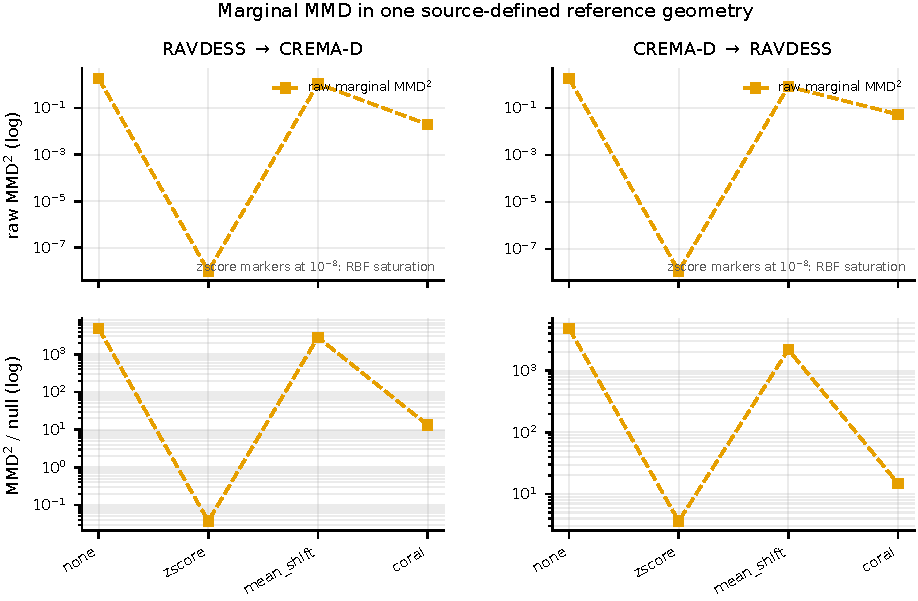
\includegraphics[width=\textwidth]{decomposition.pdf}
  \caption{Marginal MMD$^2$ across the alignment ladder in the common
    source-defined reference geometry. The top row shows raw MMD$^2$; the
    bottom row divides it by a same-distribution source half-split scale. The
    class-conditional values use class-specific null scales and are not divided
    by the marginal values.}
  \label{fig:s-decomposition}
\end{figure*}

\paragraph{A single fixed bandwidth can itself fail.} The z-score cells of Table~\ref{tab:decomposition}
are near zero because the scale-changing map saturates the RBF kernels under a
bandwidth fixed in the unaligned source geometry. They are not evidence that the
two distributions became identical. The table therefore documents a limitation of
both common comparison choices: an adaptive median bandwidth is scale-invariant,
while a globally fixed bandwidth can saturate. This is the concrete instance
behind the article's measurement-geometry argument.

\section*{S5. CORAL's shrinkage trajectory}
\label{sec:s-eps}

The article states the analytic limit: with each covariance regularised as
$C + \varepsilon\,\mathrm{tr}(C)/d \cdot I$, CORAL's map satisfies
\begin{equation}
  M \;\longrightarrow\; \sqrt{\mathrm{tr}(C_t)/\mathrm{tr}(C_s)} \; I
  \label{eq:s-coral-limit}
\end{equation}
as $\varepsilon$ grows, so the transform collapses to a global scalar rescale
plus a mean shift. Table~\ref{tab:eps} and Figure~\ref{fig:s-eps}
measure the approach on real features.

The relative distance from the fitted map to the nearest scaled identity,
$\lVert M - cI \rVert / \lVert M \rVert$, falls monotonically from $0.9254$ at
$\varepsilon = 10^{-4}$ to $0.0049$ at $\varepsilon = 1000$, and the fitted
scalar converges on the predicted limit (ratio $2.195 \rightarrow 1.000$). At
$\varepsilon = 10$, selected on \texttt{source\_val} in this probe, the relative
matrix residual is $0.1436$. Empirically, \texttt{source\_val} and target
macro-F1 at $\varepsilon = 1000$ land within $0.0061$ of \texttt{mean\_shift} in
both directions.

The map limit is classifier-independent. The selected shrinkage and the observed
score proximity are not: both depend on the fitted head and the selection
protocol. This probe does not show that source validation generally drives CORAL
to that endpoint.

\begin{table}[tb]
  \centering
  \caption{CORAL's shrinkage asymptote. As $\epsilon$ grows the regularised covariances approach a scaled identity, the map tends to $\sqrt{\mathrm{tr}(C_t)/\mathrm{tr}(C_s)}\,I$, and the rung degenerates to a scalar rescale plus a mean shift. Both columns converge on \texttt{mean\_shift}.}
  \label{tab:eps}
  \begin{tabular}{lrrr}
    \toprule
    pair & $\epsilon$ & source\_val & target macro-F1 \\
    \midrule
    RAVDESS $\rightarrow$ CREMA-D & 0.0001 & 0.5177 & 0.3818 \\
     & 0.01 & 0.5693 & 0.3810 \\
     & 0.1 & 0.6273 & 0.3883 \\
     & 1 & 0.6897 & 0.4023 \\
     & 10 & 0.7235 & 0.4118 \\
     & 100 & 0.7276 & 0.3992 \\
     & 1000 & 0.7282 & 0.3879 \\
     & \texttt{mean\_shift} & \textbf{0.7278} & \textbf{0.3932} \\
    CREMA-D $\rightarrow$ RAVDESS & 0.0001 & 0.4542 & 0.4324 \\
     & 0.01 & 0.5008 & 0.4139 \\
     & 0.1 & 0.5636 & 0.4061 \\
     & 1 & 0.6257 & 0.4322 \\
     & 10 & 0.6490 & 0.4665 \\
     & 100 & 0.6517 & 0.4749 \\
     & 1000 & 0.6505 & 0.4695 \\
     & \texttt{mean\_shift} & \textbf{0.6517} & \textbf{0.4634} \\
    \bottomrule
  \end{tabular}
  \\[2pt]
  \begin{minipage}{\linewidth}\footnotesize Filter: hubert, \{logreg, svm\_rbf, mlp\} $\times$ \{last, layer:6\}, 5 seeds. $\epsilon \leq 10$ is the frozen Stage 2 grid; $\epsilon \in \{100, 1000\}$ is a 120-run off-grid probe carrying the same facet hashes. Means over seeds.\end{minipage}
\end{table}


\begin{figure*}[!t]
  \centering
  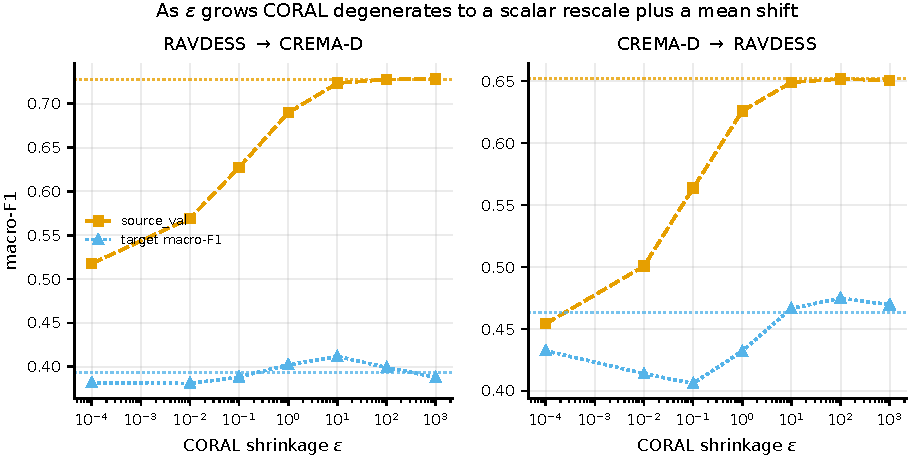
\includegraphics[width=\textwidth]{eps_asymptote.pdf}
  \caption{\texttt{source\_val} and target macro-F1 against CORAL's shrinkage
    $\varepsilon$. Dotted lines mark \texttt{mean\_shift}; the analytic map limit
    in Equation~\eqref{eq:s-coral-limit} is a scalar-rescaled mean shift. Both
    curves approach the \texttt{mean\_shift} scores.}
  \label{fig:s-eps}
\end{figure*}

\section*{S6. Per-class transfer and confusion structure}
\label{sec:s-perclass}

Table~\ref{tab:perclass} gives per-class F1 of the source-validated
configuration, computed from the stored per-utterance predictions. \texttt{sad} and \texttt{happy} fall below the macro
average in \emph{both} directions: \texttt{sad} at $0.2800$ $[0.1897, 0.3687]$
and $0.2411$ $[0.1779, 0.3028]$, \texttt{happy} at $0.3288$ $[0.1952, 0.3993]$
and $0.3618$ $[0.2759, 0.4304]$, against macro averages of $0.3335$ and
$0.5034$. A class failing in both directions is a property of the label rather
than of one corpus being the source. No class collapsed to zero predictions in
any pair. The remaining classes reorder between directions: \texttt{fear} is the
strongest reverse class at $0.6777$ $[0.6298, 0.7241]$ but is below the macro
average forward at $0.3339$ $[0.2460, 0.3733]$.
Figure~\ref{fig:s-perclass} plots the per-seed values and
Figure~\ref{fig:s-confusion} the associated row-normalised confusions.

\begin{table}[tb]
  \centering
  \caption{Per-class F1 of the source-validation-selected configuration in both transfer directions, from stored per-utterance predictions. \texttt{sad} and \texttt{happy} fall below the macro average in both directions.}
  \label{tab:perclass}
  \begin{tabular}{lrrrr}
    \toprule
    class & $n$ & F1 (RAV $\rightarrow$ CRE) & $n$ & F1 (CRE $\rightarrow$ RAV) \\
    \midrule
    \texttt{angry} & 3144 & 0.4404 [0.2974, 0.5145] & 480 & 0.5775 [0.4827, 0.6659] \\
    \texttt{disgust} & 3144 & 0.3626 [0.3249, 0.4328] & 480 & 0.5745 [0.5246, 0.6283] \\
    \texttt{fear} & 3144 & 0.3339 [0.2460, 0.3733] & 480 & 0.6777 [0.6298, 0.7241] \\
    \texttt{happy} & 3144 & 0.3288 [0.1952, 0.3993] & 480 & 0.3618 [0.2759, 0.4304] \\
    \texttt{neutral} & 2691 & 0.2551 [0.1652, 0.3149] & 720 & 0.5879 [0.5155, 0.6518] \\
    \texttt{sad} & 3144 & 0.2800 [0.1897, 0.3687] & 480 & 0.2411 [0.1779, 0.3028] \\
    \textbf{macro} &  & \textbf{0.3335 [0.2550, 0.3856]} &  & \textbf{0.5034 [0.4675, 0.5361]} \\
    \bottomrule
  \end{tabular}
  \\[2pt]
  \begin{minipage}{\linewidth}\footnotesize Filter: validated configuration per (pair, seed), 5 seeds, predictions pooled. Paired cluster bootstrap over target-test speakers and seeds, 2000 replicates. Precision and recall are in \texttt{reports/per\_class.md}.\end{minipage}
\end{table}


\begin{figure*}[!t]
  \centering
  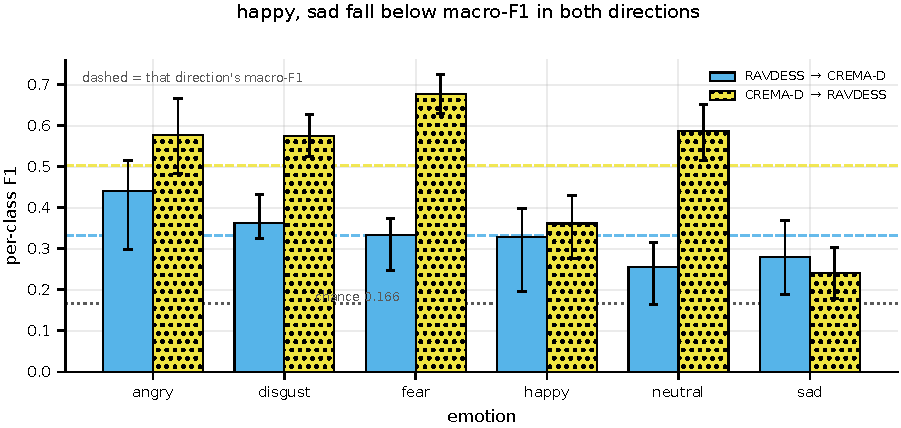
\includegraphics[width=\textwidth]{per_class_f1.pdf}
  \caption{Per-class F1 from the configuration selected on source-side
    validation for each seed, in both directions, with 95\% intervals. Dashed
    lines mark each direction's macro average; the dotted line marks the chance
    baseline.}
  \label{fig:s-perclass}
\end{figure*}

\begin{figure*}[!t]
  \centering
  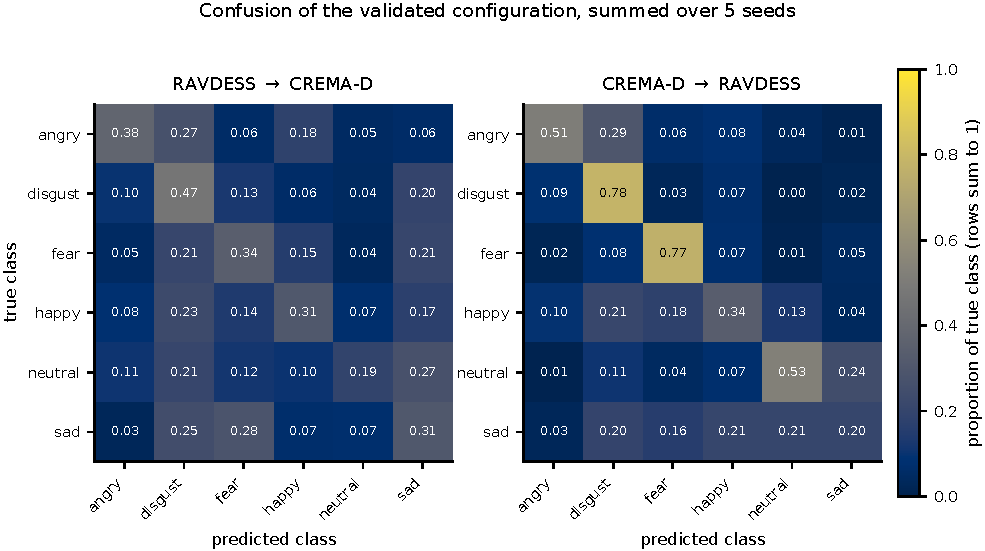
\includegraphics[width=\textwidth]{confusion.pdf}
  \caption{Row-normalised confusion from the configuration selected on
    source-side validation for each seed, summed over five seeds. Rows are true
    classes and columns predicted classes, in the alphabetical order used
    throughout.}
  \label{fig:s-confusion}
\end{figure*}

\section*{S7. Blending toward the unaligned features}
\label{sec:s-blending}

Interpolating between aligned and original features,
$\alpha \cdot x_{\text{aligned}} + (1 - \alpha) \cdot x_{\text{original}}$, was
proposed in an earlier version of this work with $\alpha$ never searched. We
searched it on the two rungs that move the features most. It is retained here as
a historical probe: it lies outside the article's central argument, and no
statement in the article depends on it.

Performance increases monotonically in $\alpha$ in the forward direction, from
$0.2987$ $[0.2746, 0.3188]$ at $\alpha = 0$ to $0.4012$ $[0.3802, 0.4186]$ at
$\alpha = 1$ for CORAL. The reverse direction rises from $0.3154$
$[0.2513, 0.3868]$ to $0.3833$ $[0.3522, 0.4225]$ but dips before it climbs.
\textbf{The best setting of the blending parameter is the one that turns
blending off}, in both directions and on both rungs, so blending is reported as
a negative result rather than as a method.

\paragraph{Does the dip survive correction?} On one rung, yes. Two adjacent steps
in the reverse direction run the wrong way, both at
$\alpha = 0 \rightarrow 0.25$. Each is tested paired on the same resampled
speakers and seeds, with Holm correction across the two. On \texttt{mkmmd\_full}
the step is $-0.0195$ $[-0.0420, -0.0020]$, $p = 0.0120$ raw and $0.0240$
corrected, which survives; on \texttt{coral} it is $-0.0142$
$[-0.0330, +0.0029]$, $p = 0.0920$, which does not. The reverse direction's
interior is therefore non-monotone in at least one place, reported as such
rather than rounded to a cleaner story. It remains a weak result: 288 runs, one
backbone, two seeds, a 624-utterance target test set, and outside the
pre-specified comparison family.

\section*{S8. MK-MMD implementation and its acceptance check}
\label{sec:s-mkmmd}

The two MK-MMD rungs learn an affine map by gradient descent on a multi-kernel
MMD objective, warm-started from CORAL. An unpenalised finite-sample MMD check
then accepts or rejects the fitted candidate against its warm start.

Optimisation uses Adam \cite{kingma2015adam} for 200 steps at batch size 256.
The learning rate is $\eta = \eta_0 / \sqrt{P}$ with $\eta_0 = 0.01$ and $P$ the
parameter count: Adam normalises per parameter, so a fixed rate would give a
step whose Frobenius norm grows as $\sqrt{P}$, reaching $\approx 0.77$ per
iteration for a full $W$, which does not converge. The identity anchor in the
objective penalises $W - I$ and not $b$, so even an ideal large-$\lambda$ limit
leaves a translation to optimise and does not necessarily recover
\texttt{none}. No asymptotic optimisation guarantee is claimed for the
finite-step procedure.

The check rejects the fitted candidate in $64.9\%$ of diagonal-map runs and
$55.2\%$ of full-map runs. In those cells the returned map is the diagonal
moment match or the CORAL warm start respectively, not a converged MK-MMD
solution. This materially qualifies the article's statement that the evaluated
MK-MMD conditions do not outperform the simpler rungs: that statement is about
this complete finite procedure, including its fallback, and not about every
possible optimiser or every affine MK-MMD solution. Rejection under an
unpenalised check is also not proof that the penalised training objective failed
to improve.

\section*{S9. Provenance ledger of withdrawn claims}
\label{sec:s-provenance}

This ledger records claims made during the project that were later withdrawn,
narrowed or reversed by additional evidence. It preserves the research history
without using any withdrawn statement as support for the article.

\begin{itemize}
  \item \emph{``Z-scoring removes 97.6\% of marginal MMD, more than CORAL.''}
    \textbf{Retracted}: this was a per-rung bandwidth artefact. Under a fixed
    bandwidth, CORAL reached $2.0\times$ the null against \texttt{zscore}'s
    $31.3\times$. This led to the article's measurement-geometry analysis.
  \item \emph{``The cheapest step does all the work.''} \textbf{Retracted}:
    a one-seed result over-read a $0.019$ spread. The article instead uses the
    bounded five-seed ladder comparison.
  \item \emph{``Target macro-F1 is flat across $226\times$ of discrepancy.''}
    \textbf{Refuted}. In the measured final-layer condition, alignment adds
    $+0.084$ forward and $+0.128$ reverse at five seeds.
  \item \emph{``\texttt{layer:6} has lower discrepancy than \texttt{last} and
    transfers worse.''} \textbf{Partly refuted}: the discrepancy comparison
    does not reproduce under the corrected MMD protocol; the transfer result
    survives only for the unaligned forward condition.
  \item \emph{``In-domain-optimal depth is 4--5 layers shallower in all three
    backbones.''} \textbf{Retracted}. The pooled 36-cell gap is $+0.00$ layers
    $[-0.57, +0.57]$. The effect remains only at rung \texttt{none}, forward,
    at $+4.2$, $+4.2$ and $+2.4$ layers.
  \item \emph{``Selecting depth on \texttt{source\_val} systematically picks
    the wrong depth.''} \textbf{Contradicted}. Against a random layer,
    \texttt{source\_val} is better by $-0.0366$ $[-0.0448, -0.0285]$.
    Source validation is therefore informative for depth but not for the
    alignment decision in the forward direction.
  \item \emph{``Extending the $\varepsilon$ grid would move the argmax
    again.''} \textbf{Falsified}. The probe saturates, and the CREMA-D to
    RAVDESS argmax is interior at $\varepsilon = 100$.
\end{itemize}

Frame dependence was first promoted on two-seed evidence, then demoted when
the ladder axis agreed, and confirmed at full seed count on the layer axis.
The article reports only the re-specified result: the discrepancy--transfer
relationship is not invariant to the stated basis and bandwidth rule.

\bibliographystyle{cas-model2-names}
\bibliography{refs}

\end{document}
